\documentclass{beamer}
\usepackage{graphicx}
\usepackage{amsmath}
\usepackage{amssymb}
\usepackage{amscd} % Required for inserting images
\usetheme{metropolis}
\metroset{block=fill} 

\title{Modelisation d'Aptemeres d'ADN IFT 3710}
\author{Dereck Piché, Jonas Gabirot, Guillermo Martinez}
\institute{Universite de Montreal}
\date{Mars 2023}


\begin{document}

\frame{\titlepage}

\
\section{Contexte}

\begin{frame}{Contexte}

\end{frame}


\section{Transformeurs}

\begin{frame}{Attention}
Un système d'attention retourne une somme des vecteurs \emph{Valeurs} selon 
une mesure de similarité entre les vecteurs \emph{Requêtes} et les vecteurs \emph{Clés}.
Cette mesure de similarité est appelée l'attention.
    \begin{block}{Système d'attention}
        $\sum_{j} a(q, k_j) v_j$
    \end{block}
Les transformeurs utilisent un système d'auto-attention, qui vise à produire
une séquence transformée ou`' chaque jeton est codé en effectuant une somme pondérée des
autres jetons présents dans sa séquence (l'incluant).
    \begin{block}{Jeton codé}
        $t_{i}^{'} = \sum_{j} a(W^{q}t_{i}, W^{k}t_j) W^{v}t_j$
    \end{block}
\end{frame}

\begin{frame}{Attention}
Dans les transformeurs, on utilise une attention spéciale:
\begin{block}{Attention au produit scalaire mis à l'échelle}
    \[ a(q, k) = softmax( \frac{q^Tk}{\sqrt{d}}) \]
\end{block}


{\bf Pourquoi le produit scalaire?}
On sait déjà que le produit scalaire peut être vu comme une mesure de la similarité entre
les deux vecteurs. Cela permet beaucoup de liberté au transformeur, qui obtient les vecteurs clés et les vecteurs requêtes en fonction des vecteurs jetons avant d'effectuer le produit scalaire. On le laisse donc créer sa propre mesure de distance, en quelque sorte.

\end{frame}

\begin{frame}{}
    
{\bf Pourquoi le softmax?}
La fonction softmax assure que les coefficients sommeront à 1. Donc, on assure que les 
vecteurs de sortie de l'attention ne seront pas saturés. Ils n'auront pas des normes gigantesques pouvant causer des erreurs numériques. On peut aussi intuitivement voir l'intuition d'attention pour les coéfficients normalisés à 1.

{\bf Pourquoi la division par la racine de la taille? }
Pour éviter des erreurs numériques. On épargne les détails.

\end{frame}

\begin{frame}{Couche de codage}
    Une tête d'attention retourne donc une séquence de la même taille que son entrée (sauf exceptions).
    Une couche de codage contient plusieurs têtes d'attention! Les sorties de ces 
    têtes d'attention sont concaténées dans {\it un gros vecteur} et on applique une transformation 
    linéaire (avec activation ReLU pour obtenir de l'expressivité non linéaire) à ce vecteur pour obtenir une sortie 
    de dimension arbitraire.
\end{frame}

\begin{frame}{Architecture du transformeur}
\begin{equation*}
    \begin{CD}
        @. Seq \in R^{30}
        @>Emb.>> 
        @>Cod. (\times 3)>> 
        @>Lin.>> 
        @>ReLU>> Seq \in R
    \end{CD}
\end{equation*}

\begin{block}{Hyperparamètres}
\begin{enumerate}
    \item Taux d'apprentissage:
    \item Nombre de paramètres: 1 786 753 
    \item Codage positionnel: Sin Cos du papier TODO
\end{enumerate}
\end{block}
\end{frame}


\begin{frame}{Résultats du transformeur}
\begin{figure} \label{fig:transformer_accuracy}
    \caption{Précision du transformeur selon MSE} \center
    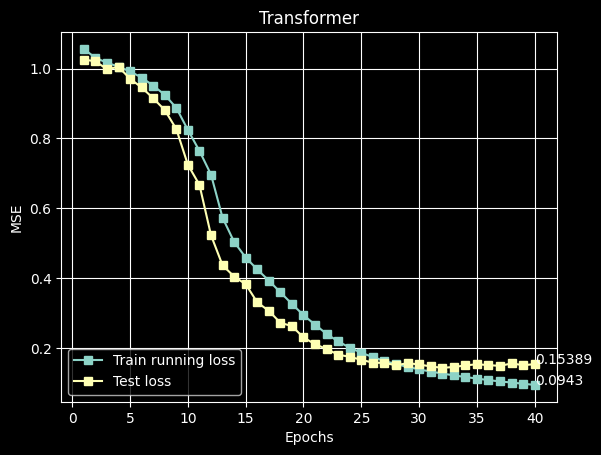
\includegraphics[width=0.7\textwidth]{images/2023-04-02-13-48-49.png}
\end{figure}

\begin{figure}
     \center
    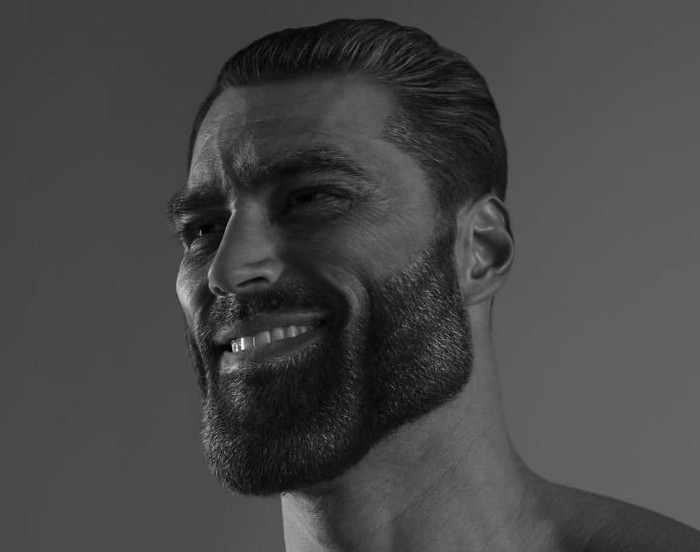
\includegraphics[width=0.1\textwidth]{images/2023-04-02-18-02-45.png}
\end{figure}
\end{frame}


\end{document}

